\documentclass[a4paper,12pt]{article} 
\usepackage{enumitem}
\usepackage{color}
\usepackage{graphicx}
\usepackage{float}
\usepackage{minted}
\usepackage{hyperref}
\usepackage[parfill]{parskip}
% End loading packages

\newcommand{\bck}{
    \textbackslash
}
\newcommand{\iph}[2]{
    \includegraphics[width=#1\textwidth,height=#1\textheight,keepaspectratio]{#2}
}
\newcommand{\ph}[1]{
    \includegraphics[width=0.5\textwidth,height=0.5\textheight,keepaspectratio]{#1}
}
\newcommand{\ita}[1]{
    \textit{#1}
}
\newcommand{\bfa}[1]{
    \textbf{#1}
}
\newcommand{\swastik}[1]{%
    \begin{tikzpicture}[#1]
        \draw (-1,1)  -- (-1,0) -- (1,0) -- (1,-1);
        \draw (-1,-1) -- (0,-1) -- (0,1) -- (1,1);
    \end{tikzpicture}%
}
\newcommand{\dph}[3]{
\begin{figure}[H]
  \centering
  \iph{#1}{#2}
  \caption{#3}
\end{figure}
}

\newcommand{\oph}[2]{
\begin{figure}[H]
  \centering
  \iph{0.78}{#1}
  \caption{#2}
\end{figure}
}
% End setting basic commands

\setminted{breaklines=true, tabsize=2, breaksymbolleft=}

% End setting basic settings.

\begin{document}
\title{Database Design And Implementation For E-Commerce}
\author{\small{Sourabh Aggarwal (111601025), Nikhil Kumar Yadav (111601013)}}
\date{\today}
\maketitle
\pagenumbering{roman}
\tableofcontents
\newpage
\pagenumbering{arabic}

\section{Contribution}
We both (Nikhil and Sourabh) agree with each other that we have contributed equally to this project. 

We both sat and discussed the project outline and we divided the work among us equally. We regularly consulted each other throughout the development phase.

\section{Introduction}
In this project, our aim was to come up with a reasonably scalable database along with basic GUI for E-Commerce purpose.

We started by listing down various requirements presented in the next section. After that we proceeded on building an ER Diagram to fullfil the same. After that it was time to implement all this in SQL. In due time, we managed to put various important features provided by almost all E-Commerce site in our project. 

So the following report touches on each of these aspects in brief and sequential manner. 

\section{Requirements}
Following is the list of requirements.
\begin{enumerate}
  \item Idea of roles. Model should have role for each of Customer, Seller and Shipper. Each user is thus assigned its role.

  \item Company maintains the details of it users like their name, address, phone number and email-id.

  \item Each user has security credentials like their username and password.
  \item It should be possible for each user to update their information including their password.
  \item Customer requirements
  \begin{enumerate}
    \item Customers should be able to browse all products.
    \item They should be able to add those products in their cart. Thus each Customer should possess a cart into which they can add products for purchasal.
    \item Note that each product could be sold by different sellers, so customer should be able to select a product corresponding to the seller they wished to buy from. 
    \item Once all the items are added in cart, Customer should then be able to purchase all those items in cart at once.
    \item For each of the product the Customer has bought, it should be possible for customer to pass the rating and review for both the product as well as seller. 
  \end{enumerate}

  \item Seller requirements
  \begin{enumerate}
    \item Each Seller possesses a rating which they should be able to see. This rating is given and updated by the users of role Customer who purchased the product from Seller.
    \item Seller should list down the products they are willing to sell. Each product should have:
    \begin{enumerate}
      \item Product Name
      \item Product Image
      \item Price 
      \item Quantity which the seller possess of the product
      \item Pickup address
      \item Description
      \item Rating (Product rating is again updated by the users of role Customer)
    \end{enumerate}
    \item It should be possible for seller to add or update his or her products.
    \item It should be possible for seller to see his or her past sellings.
    \item It should be possible for seller to see the products which they has listed. 
    \item It should be possible for seller to see their earnings in a specific duration. 
    \item Seller should be able to browse Shippers so that they can decide and contact various Shippers.
    \item It should be possible for seller to see the latest purchasal's of his or her products which are pending to be shipped, thus seller should also have an interface to update customer with the sold product's shipment Tracking ID.
  \end{enumerate}
  \item Shipper requirements
    \begin{enumerate}
      \item It should be possible for shipper to see his or her past shipments (using our interface) including source and destination of the product.
    \end{enumerate}
\end{enumerate}

\section{Entity Relation Diagram}
\subsection{Enhanced ERD}
Enhanced Entity Relation Diagram can be represented in various notations, below shows the notation which we have followed.


\begin{figure}[H]
    \centering
    \iph{0.5}{ERDNotation}
    \caption{Entity Relation Diagram Notation}
\end{figure}

Following this notation, our ERD is represented below.

\begin{figure}[H]
    \centering
    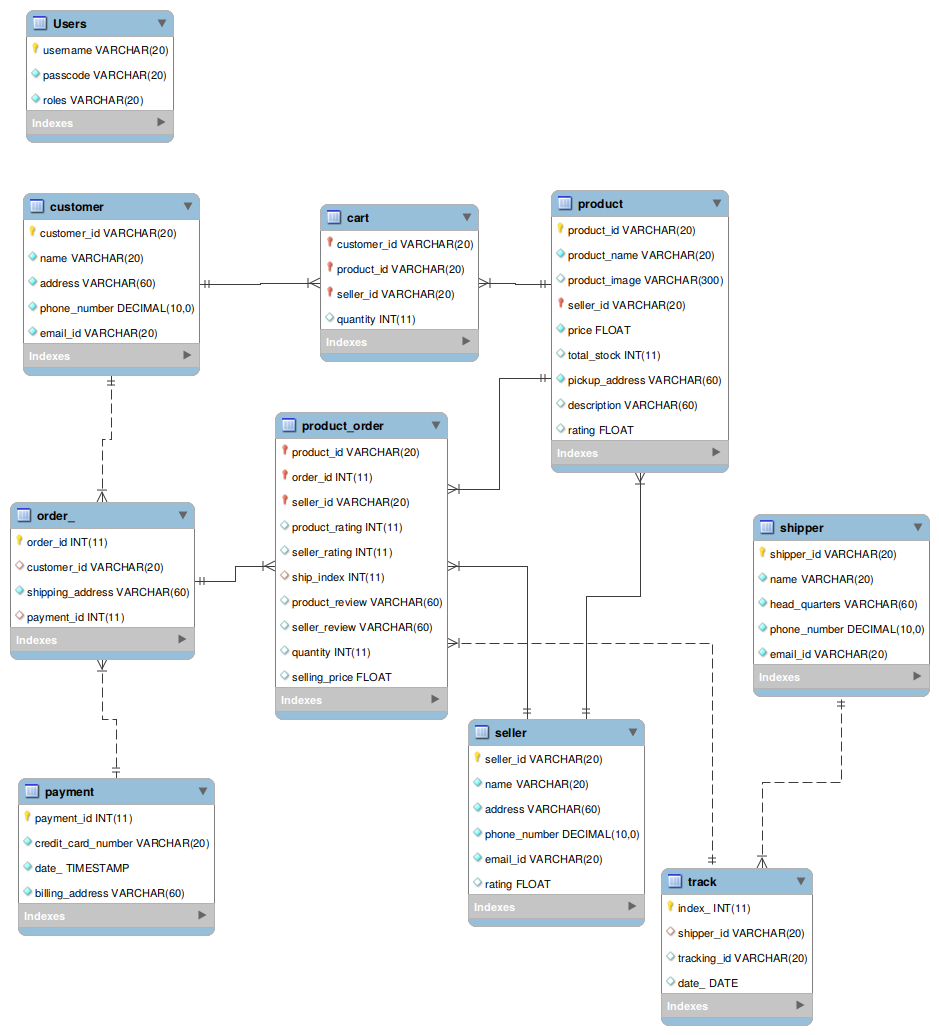
\includegraphics[width=1\textwidth]{ERDL} 
    \caption{Entity Relationship Diagram for e-commerce}
\end{figure}
\textit{Note :} The dotted line is to show that the foreign key used to draw that line is not primary key (or part of primary key) in one of the two tables.

\subsection{Simple ERD}

\dph{1}{ERDF}{Simple Entity Relationship Diagram for e-commerce}

\section{Database Schema And Normalization}
In this section we describe various aspects of our schema and also mention that it is indeed normalized (BCNF). All sections except this don't have code but we feel it is necessary to include code in this section for better understanding of various relations. 

\ita{Notation: }A dependency $A \rightarrow B$ is called relevant if all other dependencies from $A$ are of the form $A \rightarrow C$ where $C \subseteq B$.

\begin{itemize}
  \item A table for basic details of customer.
\begin{minted}{SQL}
/*  Here: customer_id -> R is the only relevant dependency and hence it is in BCNF */
create table customer (
  customer_id VARCHAR (20) primary key not null,
  name VARCHAR (20) not null,
  address VARCHAR (60) not null,
  phone_number DECIMAL (10) UNSIGNED not null,
  email_id VARCHAR (20) not null
);
\end{minted}
  \item A table for basic details of seller.
  \begin{minted}{SQL}
/* Here: seller_id -> R is the only relevant dependency and hence it is in BCNF */
/* Rating will be updated with the help of triggers. */
create table seller (
  seller_id varchar (20) primary key not null,
  name varchar (20) not null,
  address varchar (60) not null,
  phone_number decimal (10) UNSIGNED NOT NULL,
  email_id VARCHAR (20) not null,
  rating float
);
  \end{minted}
  \item A table for basic details of shipper.
  \begin{minted}{SQL}
/*  Here: shipper_id -> R is the only relevant dependency and hence it is in BCNF  */
create table shipper (
  shipper_id varchar (20) primary key not null,
  name varchar (20) not null,
  head_quarters varchar (60) not null,
  phone_number decimal (10) UNSIGNED not null,
  email_id VARCHAR (20) not null
);

  \end{minted}
  \item Having described these basic tables, we can now describe table for products. Note that each product can be sold by different sellers in different price and quantity, thus, primary key is formed by both product\_id and seller\_id. 
  \begin{minted}{SQL}
/*  Here: (product_id, seller_id) -> R is the only relevant dependency and hence it is in BCNF  */
/* Rating will be updated with the help of triggers. */
create table product (
  product_id varchar (20) not null,
  product_name varchar (20) not null,
  product_image varchar(300),
  seller_id varchar (20) not null,
  price float not NULL,
  total_stock int,
  pickup_address varchar (60) not null,
  description varchar (60),
  rating float,
  foreign key (seller_id) references seller (seller_id) on delete cascade,
  primary key (product_id, seller_id)
);

  \end{minted}
  \item When user makes a payment, we want to store payment details for which we have the following table.
  \begin{minted}{SQL}
/*   Here: payment_id -> R is the only relevant dependency and hence it is in BCNF  */
create table payment (
  payment_id int AUTO_INCREMENT primary key not null,
  credit_card_number VARCHAR (20) not null,
  date_ timestamp,
  billing_address varchar(60) not null
);
    
  \end{minted}
  \item User will have a front end feature to add items in cart. When the user is ready to buy, it will generate an \ita{order\_id} for all those products which they chose. Note that \ita{order\_id} will be generated \ita{only} when user successfully does the payment.
  \begin{minted}{SQL}
/* Here: order_id -> R is the only relevant dependency and hence it is in BCNF  */
/* Initially payment id can be null and then later once the customer does the payment, trigger will add the payment id */
create table order_ (
  order_id int AUTO_INCREMENT primary key not null,
  customer_id VARCHAR (20),
  shipping_address varchar(60) not null,
  payment_id int,
  foreign key (customer_id) references customer (customer_id) on delete set null,
  foreign key (payment_id) references payment (payment_id) on delete set null
);
  \end{minted}
  \item After generating the \ita{order\_id} (by successful completion of payment), we have to put the details of the bought items along with their \ita{order\_id}.
  \begin{minted}{SQL}
/*  Here: (product_id, order_id, seller_id) -> R is the only relevant dependency and hence it is in BCNF  */
create table product_order (
  product_id varchar(20) not null,
  order_id int not null,
  seller_id varchar (20),
  product_rating int check (product_rating in (NULL, 1, 2, 3, 4, 5)),
  seller_rating int check (seller_rating in (NULL, 1, 2, 3, 4, 5)),
  ship_index int,
  product_review varchar (60),
  seller_review varchar (60),
  quantity int,
  selling_price float,
  primary key (product_id, order_id, seller_id),
  foreign key (product_id) references product (product_id) on delete cascade,
  foreign key (order_id) references order_ (order_id) on delete cascade,
  foreign key (seller_id) references seller (seller_id) on delete cascade,
  foreign key (ship_index) references track (index_) on delete set null
);
  \end{minted}
  \item Note that we used a foreign key in the above table which we haven't defined yet, which is \ita{ship\_index}. It is basically a unique identifier for each ordered product serving as an index of track table which we will use to track our items.
  \begin{minted}{SQL}
    
/*  Here: index_ -> R is the only relevant dependency and hence it is in BCNF  */
create table track (
  index_ INT AUTO_INCREMENT primary key not null,
  shipper_id varchar (20),
  tracking_id varchar (20),
  date_ DATE,
  foreign key (shipper_id) references shipper (shipper_id) on delete set null
);
  \end{minted}
  \item A relation for \ita{cart}.
  \begin{minted}{SQL}
/*  Here: (customer_id, product_id, seller_id) -> R is the only relevant dependency and hence it is in BCNF  */
create table cart (
  customer_id varchar(20),
  product_id varchar(20),
  seller_id varchar(20),
  quantity int,
  primary key (customer_id,product_id,seller_id),
  foreign key (customer_id) references customer(customer_id) on delete cascade,
  foreign key (product_id,seller_id) references product(product_id,seller_id) on delete cascade
);
  \end{minted}
  \item We also have an auxiliary table for keeping track of users with their old passwords as mysql.user encrypts the passwords and there is no way to get it back also this table is required for validation when the user tries to log in the system.
  \begin{minted}{SQL}

-/*  Here: username -> R is the only relevant dependency and hence it is in BCNF  */
create table Users (
  username VARCHAR (20) primary key not null,
  passcode VARCHAR (20) not null,
  roles VARCHAR (20) not null
);
  \end{minted}
\end{itemize}
\newpage
\section{Roles, Views and Triggers}
\subsection{Roles}
As mentioned before, we have three roles, viz., Customer, Seller and Shipper. And of course above them all we have database administrator, "root", viz. "dbadmin". Each role will be able to access views, functions, procedures written for it and granted to it.
\subsection{Views}
Almost all what we wanted to achieve was possible with the help of procedures, views, thus have little to offer but still we are listing here all the views that we wrote irrespective of whether they are actually part of our GUI.
\subsubsection{Customer Views}
\begin{enumerate}
  \item View that will allow customer to view its profile, "customerProfile".
  \item View that will allow customer to see the total cost of his/her various orders, i.e. total money spent on the platform till date, "orderPrice". 
  \item View that will allow customer to see and add products to his cart, "showCart".
  \item View that will tell the customer details corresponding to his/her all order\_id mentioning complete order details (order\_id, shipping\_address, date\_, total\_price) except the products in that order, "previousOrders". 
  \item View that will allow customer to just see his various order\_id, "listOrders". 
  \item View that will give us shipment index (ship\_index), order ID, product ID from product\_order relation corresponding to our orders, "trackID".
  \item View that will augment the above view with tracking ID as well, "packageStatus".
\end{enumerate}
\subsubsection{Seller Views}
\begin{enumerate}
  \item View that will allow seller to view its details, "sellerProfile".
  \item View that will allow seller to see his/her various products, "sellerProducts".
  \item View that will allow seller to see various orders which they have sold (seller\_id, product\_id, quantity, selling\_price, date\_), "sellerOrders".
\end{enumerate}
\subsubsection{Shipper Views}
\begin{enumerate}
  \item View that will allow shipper to view its details, "shipperProfile".
  \item View that will allow shipping details (pickup\_address, shipping\_address, tracking\_id), "shipperTrack".
\end{enumerate}
And their details is best understood with the help of the following code:
\subsection{Triggers}
\begin{enumerate}
  \item When a product is sold, we want to mention its selling\_price as later the seller can update the price, "setPrice". (sets NEW.selling\_price entry in product\_order).
  \item When a customer passes a rating for product we have to update it in our product table, "updateRatingProduct" (update is done by averaging over all ratings).
  \item When a customer passes a rating for seller we have to update it in our seller table, "updateRatingSeller" (update is naturally done in "seller" relation by averaging over all ratings passed to our seller).
  \item When a product is sold, we need to add an entry to our track table for the same and also we have to reduct the total\_stock of that product offered by that seller. Both of these are done together by our trigger, "stockCheckandaddTrack" (naturally it will have shipper\_id, tracking\_id field NULL as of now and this info will be used to determine whether the product has been shipped or not)
  \item To check whether the products added in cart are valid or not. In case it is valid we proceed else we raise an exception. Trigger name "validCartinsert".
  \item Same as above but for update operation on cart, "validCartupdate".
\end{enumerate}
\newpage
\section{Functions And Procedures}
Below you can see details description and implementation of various Procedures and Functions, due to the nature of operations mentioned in our requirements we have preferred procedures in most cases over functions, thus if we have used function, we explicitly mention it.

\subsection{Customer Procedures}
\begin{enumerate}
  \item Procedure to see purchases between some duration, "seePurchasesByDate(IN startTime TIMESTAMP, IN endTime TIMESTAMP)" -$>$ Will return complete details from order, payment, product and product\_order table.
  \item Procedure to see items in cart, "getProductsFromCart ()" -$>$ which selects everything from view "showCart".
  \item Procedure for customer to checkout items present in cart, "purchaseEverythingInCart(IN oid varchar(20))" -$>$ which takes in order id and then for each product present in cart, will add the corresponding entry to product\_order table.
  \item Procedure for customer to remove product from cart, "removeProductCart(IN pid varchar(20), IN sid varchar(20))" -$>$ which takes in that products product\_id and seller\_id and thus delete such product from cart (deletion is performed using view showCart).
  \item Procedure for customer to update a product in cart (i.e. change quantity of the chosen product), "CREATE PROCEDURE updateProductCart(IN pid varchar(20), IN sid varchar(20), IN N INT)".
  \item Procedure for customer to make an order, "makeorder(IN cnum varchar(20), IN badd varchar(20), IN cid varchar(20), IN sadd varchar(20))" which takes a credit card number, "cnum", billing address, "badd", customer ID, "cid" and a shipping address, "sadd" and first adds an entry into payment table by selecting date using "NOW()" function and then since payment table had payment\_id which was set to automatic increment so we after fetching it insert the corresponding entries into order\_ table and then again by fetching order\_id as it was auto increment, we call already discussed procedure, "purchaseEverthingInCart".
  \item Procedure to add product to cart, "addProductToCart(IN cid varchar(20), IN pid varchar(20), IN sid varchar(20), IN q int)" which will decide whether to update the quantity if the product is already there in cart, or to add this new record into our cart.
  \item Procedure to see latest N purchases, "seeLatestNPurchases(IN N INT)" which takes in N and then gives rows corresponding to payment, order\_, product\_order, product, table and track (by taking join) ordered decreasingly by payment date.
  \item Procedure to see Purchases between dates, "seePurchasesByDate(IN startTime TIMESTAMP, IN endTime TIMESTAMP)" -$>$ works same as before just that it gives entries between the given time.
  \item Procedure to see products within price range, "queryProductsTim(IN productName varchar(20), IN lowRange FLOAT, IN highRange FLOAT)" -$>$ which after receiving suitable parameters, return entries from product sorted by price between the given range.
  \item Procedure to see reviews of a given product, "ProductReviews(IN pid varchar(20), IN sid varchar(20))" -$>$ will fetch ratings and reviews of the given product from product\_order, etc.
  \item Procedure to add review for a product, "addReviewProduct(IN pid varchar(20), IN oid varchar(20), IN sid varchar(20), IN rev varchar(60))" -$>$ as only those who have purchased successfully the product can add reviews, we need order ID for verification.
  \item Procedure to add review for a seller, "addReviewSeller(IN pid varchar(20), IN oid varchar(20), IN sid varchar(20), IN rev varchar(60))" -$>$ again we need order ID for verification. 
  \item Procedure to add rating for product, "addRatingProduct(IN pid varchar(20), IN oid varchar(20), IN sid varchar(20), IN rating INT)".
  \item Procedure to add rating for seller, "addRatingSeller(IN pid varchar(20), IN oid varchar(20), IN sid varchar(20), IN rating INT)".
  \item Procedure to see products sorted by rating, "queryProductsRat(IN productName varchar(20))".
  \item Procedure to update customer info, custUpdateInfo(IN customer\_id varchar(20), IN password VARCHAR(20), IN name varchar(20), IN address VARCHAR(60), IN phone\_number DECIMAL(10) UNSIGNED, IN email\_id VARCHAR(20)).
\end{enumerate}
\subsection{Seller Procedures}
\begin{enumerate}
  \item \textbf{Seller Function: }Function to return the total earning of a seller between supplied dates, "sellerStatsBetweenDate(startTime TIMESTAMP, endTime TIMESTAMP)".
  \item Procedure for seller to see sold but not shipped products, soldButNotShipped(IN seller\_id varchar(20)) -$>$ fetches entries from product\_order table which have corresponding shipper\_id NULL.
  \item Procedure for seller to ship a sold product, "shipSoldProduct(IN gproduct\_id varchar(20), IN gorder\_id varchar(20), IN gseller\_id varchar(20), IN gshipper\_id varchar(20), IN gtracking\_id varchar(20), IN gdate DATE)" -$>$ will ship the product (update shipper\_id and tracking\_id in track table) by taking relevant input.
  \item Procedure for seller to see his rating, "getRating(IN seller\_id varchar(20))".
  \item Procedure for seller to check whether there is already a product with given seller\_id and product\_id (this is useful when seller is adding a new product), "sellerCheckExistProd(IN product\_id varchar(20), IN seller\_id varchar(20))" -$>$ will return a row if there is a corresponding product.
  \item Procedure for seller to add new product, "addProduct(IN product\_id varchar(20), IN seller\_id varchar(20), IN product\_name varchar(20), IN product\_image varchar(300), IN price float, IN total\_stock int, IN pickup\_address varchar(60), IN description varchar(60))" -$>$ adds an entry in product table by taking suitable input details.
  \item Procedure for seller to update his specific product details, "updateProductInfo(IN product\_id varchar(20), IN seller\_id varchar(20), IN product\_name varchar(20), IN product\_image varchar(300), IN price float, IN total\_stock int, IN pickup\_address varchar(60), IN description varchar(60))" -$>$ Note that it is possible to call this procedure by giving empty string for entries whose update is not deemed fit.
  \item Procedure to update seller's info, "sellerUpdateInfo(IN seller\_id varchar(20), IN passwordd VARCHAR(20), IN named varchar(20), IN addressd VARCHAR(60), IN phone\_number DECIMAL(10) UNSIGNED, IN email\_id VARCHAR(20))" -$>$ Note that it is possible to call this procedure by giving empty string for entries whose update is not deemed fit.
  \item Procedure for seller to see his or her past sold products within a specific time duration, "seeSellingsBetweenDuration(IN startTime TIMESTAMP, IN endTime TIMESTAMP)" -$>$ fetches the relevant entries from product\_order table.
  \item Procedure to see latest N sellings, "seeLatestNSellings(IN N INT)" -$>$ fetches the relevant entries from product\_order table.
  \item Procedure to see seller's already listed similar products with increasing price, "selQuerySimProducts(IN productName varchar(20))".
  \item Procedure to see seller's similar products sorted by rating, "selQueryProductsRat(IN productName varchar(20))".
\end{enumerate}
\subsection{Shipper Procedures}
\begin{enumerate}
  \item Procedure to update shipper's info, "shipperUpdateInfo(IN shipper\_id varchar(20), IN passwordd VARCHAR(20), IN named varchar(20), IN addressd VARCHAR(60), IN phone\_number DECIMAL(10) UNSIGNED, IN email\_id VARCHAR(20))" -$>$ works in the same way as other user's update info.
  \item Procedure for shipper to see his or her past shipments within a specific time duration, "seeShipmentsBetweenDuration(IN startTime DATE, IN endTime DATE)" -$>$ fetches targeted entries from track table.
  \item Procedure to see latest N Shipments, "seeLatestNShipments(IN N INT)" -$>$ fetched targeted entries from track table.
\end{enumerate}

\section{Tour Of GUI And Use Cases}
\subsection{Login Window}
On start, user will be popped with this window where they can enter their detail, and if the credentials are incorrect message will be shown depicting the same. User need not specify their role, it will be automatically determined from our User Table. Also if the user wants to create an account, they can select "SignUp" option.

\dph{0.78}{log}{Login Window}

\subsection{Sign Up}

User can first select their role and then fill in their details, it implements various logic such as to check whether user has checked exactly one tick box, passwords match, whether the required fields are left empty, such a user already exists, etc.

\dph{0.78}{sign}{Sign Up: Select Role}

\dph{0.78}{sign2}{Sign Up: Enter Details}

\subsection{Customer Window}

Now suppose a user of role customer logs in, they would be greeted with following windows which are shown in figure.

\dph{0.66}{customer}{Customer Window}


\subsubsection{Previous Products}

Here user can chose how to see their previous products, either by date (again various logics are implemented to check whether the entered date is correct, etc.) or by giving "N" for latest "N" purchases. Users can now select a particular purchased product and give ratings, reviews, etc. They can also see shipment status.

\dph{0.99}{previousprod}{Previous Products}

\subsubsection{Browse Products}

User can browse either by searching by name which will give results in decreasing order of rating or by searching within their budget. For the selected item, they can chose how much amount to add in cart and also see previous reviews of the product.

\dph{0.99}{browseprod}{Browse Products}

\subsubsection{Cart}

Here user will be able to see items added in cart where they can update the quantity or remove the item from cart and obviously checkout from cart option is there whereby user will be asked to enter details payment details.

\dph{0.99}{cart}{Cart}

\subsubsection{Update Your Info}

Facility for User to update their profile.

\dph{0.99}{uppcust}{Update Info: Customer}

\subsubsection{View Your Profile}

Facility for User to view their profile.

\dph{0.79}{pcust}{View Profile: Customer}


\subsection{Seller Window}

Now suppose a user of role seller logs in, they would be greeted with following windows which are shown in figure.

\dph{0.66}{seller}{Seller Window}


\subsubsection{Add New Products}

Facility for seller to add a new product.

\dph{0.99}{newprod}{Add New Product}

\subsubsection{Update Existing Product}

Facility for seller to update change existing product information.

\dph{0.95}{mprod}{Update Existing Product}

\subsubsection{See Your Products}

Seller can browse their existing products sorted either by price or rating.

\dph{0.99}{seeprod}{See Your Products}

\subsubsection{See Past Sellings}

Facility for seller to see their past sellings either between some date or latest "N" sellings.

\dph{0.99}{psel}{Past Sellings}

\subsubsection{See Earnings Between Duration}

\dph{0.9}{ebd}{See Earnings Between Duration}


\subsubsection{See Your Rating}
Facility for seller to view their rating.

\dph{0.8}{kyr}{Know Your Rating}

\subsubsection{See Products Which Are Sold But Not Shipped}
Facility for seller to ship a sold but non shipped product. 

\dph{0.99}{ssp}{Products Sold But Not Shipped}

\subsubsection{Browse Shippers}

Facility for seller to see various shippers.

\dph{0.99}{bship}{Browse Shippers}

\subsubsection{Update Your Info}

Facility for User to update their profile.

\dph{0.99}{uppcust}{Update Info: Seller}

\subsubsection{View Your Profile}

Facility for User to view their profile.

\dph{0.79}{pseller}{View Profile: Seller}

\subsection{Shipper Window}

\subsubsection{Update Your Info}

Facility for User to update their profile.

\dph{0.99}{upship}{Update Info: Shipper}

\subsubsection{See Past Shipments}

Facility for shipper to see past shipments either by date or by setting latest "N" shipments. 

\dph{0.99}{spship}{Update Info: Shipper}

There is also a facility to see shipments in detail to see from where it was taken and where is to be delivered. 

\dph{0.99}{spshipd}{Update Info: Shipper}

\subsubsection{View Your Profile}

Facility for User to view their profile.

\dph{0.79}{pshipper}{View Profile: Shipper}

\newpage
\section{Further Reading And Useful Links}
\begin{center}
\begin{itemize}
  \item[\textbf{Schema: }] Complete implementation of schema, views, procedures, triggers, etc. can be found \href{https://github.com/nikhilyadv/DBMS-Lab-Project/blob/master/Schema.sql}{here}.
  \item[\textbf{GUI: }] GUI source code can be found \href{https://github.com/nikhilyadv/DBMS-Lab-Project/tree/master/GUI}{here}.
  \item[\textbf{Complete Project: }] All our work, including above can be found \href{https://github.com/nikhilyadv/DBMS-Lab-Project}{here}.
\end{itemize}
\end{center}
\end{document}